





\begin{figure}[t]

\centerline{
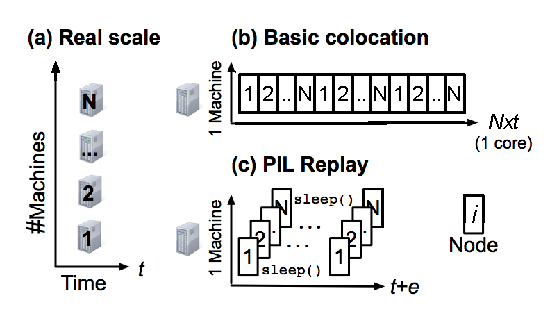
\includegraphics[height=1.75in]{F/ill/colo-hotos.eps}
%\includegraphics[height=1.75in]{F/empty.eps}
}

%\mycaption{fig-ill}{Real-scale testing, basic colocation, and scale check}{}
\mycaption{fig-ill}{Various scale-testing approaches}{The
left figure (a) illustrates a real-scale testing where the system/protocol
under test 
is deployed on $N$ machines, which illustratively takes $t$ time to complete.
%
The top figure (b) depicts a basic colocation where $N$ nodes
are packed into a single machine and exhibit CPU contention 
and context switching, which can take $N$$\times$$t$ time
to complete (in one-processor scenario).
%
The bottom figure (c) illustrates our 
processing illusion (PIL) as described in \sec\ref{sec-sck}. Here,
expensive functions are emulated with \ts{sleep()}, thus the test
time $t$$+$$e$ is similar to the real-scale testing. }


\end{figure}








\section{Scale Check}
\label{sec-sck}


We believe new methods are needed to help developers check their
systems/protocols implementation at real scale but without the hurdles of
running large test clusters.  
%
In our work, we explore a new approach to find and replay scalability bugs
in a ``cheap'' way such as on one machine, which we name {\em
  single-machine scale check} (or just ``scale check'' short).


The research question to address is: how to colocate a large number of
CPU-intensive nodes on one machine with limited resources and yet still
achieve high accuracy?
%
High accuracy implies that the colocated nodes generate a similar behavior
as if they run on independent machines.
%
The reason for inaccuracy is illustrated in Figures \ref{fig-ill}a
and \ref{fig-ill}b.
%
With real-scale testing (Figure \ref{fig-ill}a), the protocol under test
might finish in $t$ seconds.  However, with a basic colocation, the
CPU-intensive nodes contend with each other in one machine.  With only
just 1 processor core for example, the protocol under test might finish in
$N$$\times$$t$ seconds, hence the inaccuracy.
%

To address this, below we present the concept of processing
illusion (PIL) and how to find PIL-safe functions and generate output of
PIL-replaced functions.

% Figure \ref{fig-arch} depicts the major stages of our scale-check process:
% offensive function finder \textcircled{b}, memoizer \textcircled{d}, and
% replayer \textcircled{f}.



% Scalable debug time implies that the replay process can make the
% scalability bugs surface in a similar time frame ($t$$+$$\epsilon$) as in
% the real deployment ($t$), as compared in Figures \ref{fig-ill}c and
% \ref{fig-ill}a.



% Figure \ref{fig-arch} depicts the major stages of our scale-check process:
% offensive function finder \textcircled{b}, memoizer \textcircled{d}, and
% replayer \textcircled{f}.
%
% We describe each stage below in conceptual order, along with their
% technical challenges.







\def \fgw {0.85in}


\begin{figure*}[t]

\centerline{
%\includegraphics[height=\fgw]{F/empty.eps}
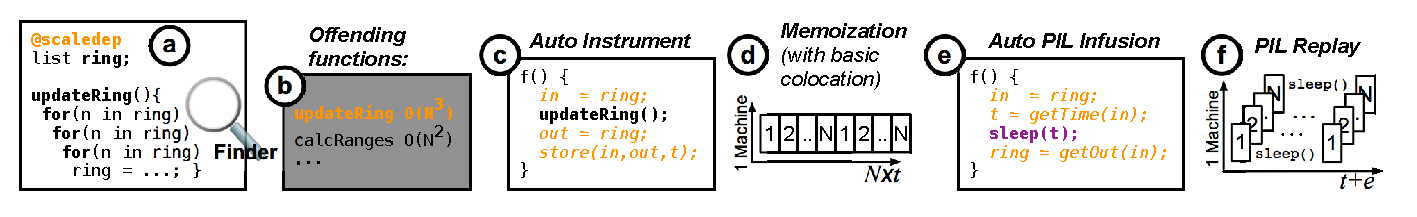
\includegraphics[height=\fgw]{F/ill/sck1-hotos.eps}
}

\mycaption{fig-arch}{The proposed flow of an automated scale-check process}{}

\end{figure*}




% --------------------------------------------
\vnb\ {\bf Processing Illusion (PIL)}
%
To achieve accuracy, we must address the CPU contention delays
($N$$\times$$t$) in basic colocation (Figure \ref{fig-ill}b).
%
We propose  emulating CPU-intensive processing with {\em
  processing illusion} (PIL), which replaces an actual processing with
\sleep.
%
With PIL, an expensive function will sleep and wake up in accurate time
with the correct output.
% thus reducing contention delays and making
%replays fast (Figure~\ref{fig-ill}c).
%
As illustrated in Figure \ref{fig-ill}c, if some computations can be
emulated with \ts{sleep()} and the output data is automatically generated
given the input data, then the resulting time is more accurate ($t$$+$$e$)
to the one in real-scale testing.



PIL extends the intuition behind data-space emulation
\cite{Wang+14-Exalt}, where the insight is: ``how data is processed is not
affected by the content of the data being written, but only by its size.''
%
For PIL, our insight is that {\em ``the key to computation is not the
  intermediate results, but rather the execution time and eventual
  output.''}
%
In other words, what matters is the global cascading implication of the
long execution time of the individual nodes.


% ---------------------------------------------
\vnb {\bf Finding PIL-safe and offending functions:} One key question PIL
method raises is: which functions can be safely replaced with \sleep
\textit{without} changing the whole processing semantic?  We name them
``PIL-safe functions/code blocks.''
%
We set a rule that a PIL-safe function must have a memoizable output (\ie,
a deterministic output on a given input) and not have any side effects
such as disk I/Os, network messages, and blocking mechanisms such as
locks.  
%
Many functions satisfy the rule above, but not all PIL-safe functions
should ``take the PIL''; that is, they might not be the ``offending''
functions that lead to scalability bugs.  Thus, we raise another key
question: which functions are offending?


We learned that many offending functions contain loops that are
cluster-size dependent (\eg, a \ts{for}-loop that iterates a cluster-ring
data structure).  Some of the loops can also be a nested loop.
%
Finding such code blocks are unfortunately not straightforward.
Scale-dependent loops can span across multiple functions; in \caone,
$O(N^3)$ loops span 1000+ LOC across 9 functions.  Moreover, they can be
inside some \ts{if-else} branches reachable only from a certain
path/workload; in \caone, the last $O(N^2)$ loop is only exercised
if the cluster bootstraps from scratch.
%
All of these suggest that finding PIL-safe and offending functions require
an advanced program analysis (which we discuss later).  Such a tool will
guide the developers to decide which paths/protocols to test, to uncover
potential scalability bugs.




% -----------------------------------
\vnb {\bf Memoizing PIL-replaced functions:} PIL-safe and offending
functions will become ``PIL-replaced functions'' where their actual
processing will be skipped during replays with \ts{sleep(t)}.
%
Thus, two more questions to address are: how to produce the output if the
actual computation is skipped and how to predict the actual compute time
(\ts{t}) accurately?


The answer to the first question is {\em pre-memoization}.  That is, given
a PIL-replaced code block, we need to first execute the code block and
record the input/output around it.
%
The only way to do this on a single machine is to run the protocol with
basic colocation, which will consume some time due to the CPU contention
delays.
%
However, this will only be a {\em one-time} overhead, while the fast
PIL-infused replay stage can be repeated numerous times without
contention.



It is challenging to pre-memoize PIL-replaced functions with an offline
input-sampling method without running the protocol at least once.
%
The reason is that, in the context of large-scale, decentralized,
non-deterministic distributed systems, covering all possible input/output
pairs may require an ``infinite'' time and storage space.
%
In other words, input/output pairs depend on the precise order of message
arrivals, which can be random.
%
In a ring rebalancing algorithm for example, with $N$ nodes and $P$
partitions/node, there are $(N^{NP})^2$ input/output pairs given all
possible orderings.
%
Thus, to cap the state space, the pre-memoization stage also records
message ordering, which will be deterministically enforced during
PIL-infused replay.  With this ``order determinism,'' we do not have to
record all possible input/output pairs.  We simply record pairs that are
observed in one particular run of the protocol test.

% then the replay stage enforces order determinism.

The answer to the second question (predicting \ts{t}) is {\em in-situ time
  recording}; in addition to storing input/output pairs we also store
input/duration pairs (Figure \ref{fig-arch}c).
%
It is almost impossible to predict compute time with a
prediction/static-analysis approach.
%
As mentioned above, nested loops can span across multiple functions with
many \ts{if-else} conditions.  In a Cassandra bug, the duration of an
offending code block can range from 0.001 to 4 seconds depending on 
multi-dimensional inputs.
%
One might also wonder whether time recording is enough to hint the
developers of the potential scalability bugs (\eg, 4 seconds of compute
should raise a red flag).
%
As mentioned earlier, every implementation is unique (\sec\ref{sec-chal});
for example, in \ca{5456}, if the lock is fine-grained, the long compute
will not cause cascading impacts.
%
Furthermore, patches of scalability bugs do not always remove the
expensive computation.
%
Put simply, scalability bugs are not merely about the expensive functions,
but rather their global implications.





